\documentclass{standalone}
\usepackage{tikz}
\usetikzlibrary{patterns, positioning}


\begin{document}
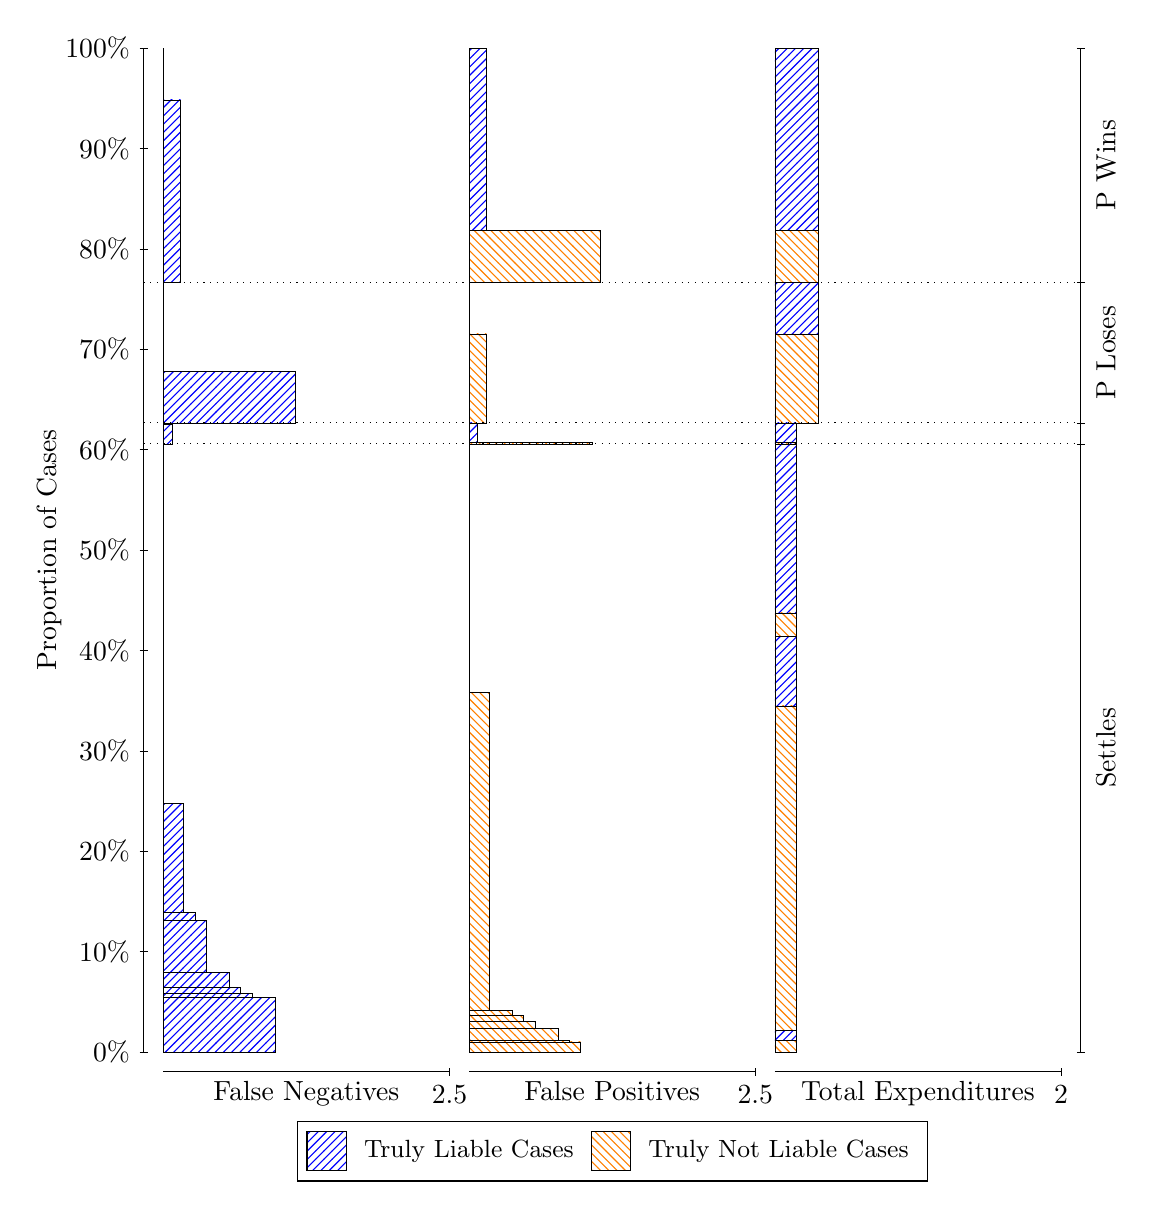
\begin{tikzpicture}
\draw[black, very thin] (1.5,1.75) -- (1.5,14.5);
\node[rotate=90, text=black, anchor=center] at (0.3, 8.125) {Proportion of Cases};
\draw[black, very thin] (1.45,1.75) -- (1.55,1.75);
\node[text=black, anchor=east] at (1.45, 1.75) {0\%};
\draw[black, very thin] (1.45,3.025) -- (1.55,3.025);
\node[text=black, anchor=east] at (1.45, 3.025) {10\%};
\draw[black, very thin] (1.45,4.3) -- (1.55,4.3);
\node[text=black, anchor=east] at (1.45, 4.3) {20\%};
\draw[black, very thin] (1.45,5.575) -- (1.55,5.575);
\node[text=black, anchor=east] at (1.45, 5.575) {30\%};
\draw[black, very thin] (1.45,6.85) -- (1.55,6.85);
\node[text=black, anchor=east] at (1.45, 6.85) {40\%};
\draw[black, very thin] (1.45,8.125) -- (1.55,8.125);
\node[text=black, anchor=east] at (1.45, 8.125) {50\%};
\draw[black, very thin] (1.45,9.4) -- (1.55,9.4);
\node[text=black, anchor=east] at (1.45, 9.4) {60\%};
\draw[black, very thin] (1.45,10.675) -- (1.55,10.675);
\node[text=black, anchor=east] at (1.45, 10.675) {70\%};
\draw[black, very thin] (1.45,11.95) -- (1.55,11.95);
\node[text=black, anchor=east] at (1.45, 11.95) {80\%};
\draw[black, very thin] (1.45,13.225) -- (1.55,13.225);
\node[text=black, anchor=east] at (1.45, 13.225) {90\%};
\draw[black, very thin] (1.45,14.5) -- (1.55,14.5);
\node[text=black, anchor=east] at (1.45, 14.5) {100\%};

\draw[black, very thin] (13.4,1.75) -- (13.4,14.5);
\draw[black, very thin] (13.35,1.75) -- (13.45,1.75);
\node[anchor=west] at (13.35, 1.75) {};
\draw[black, very thin] (13.35,9.4727) -- (13.45,9.4727);
\node[anchor=west] at (13.35, 9.4727) {};
\draw[black, very thin] (13.35,9.74) -- (13.45,9.74);
\node[anchor=west] at (13.35, 9.74) {};
\draw[black, very thin] (13.35,11.525) -- (13.45,11.525);
\node[anchor=west] at (13.35, 11.525) {};
\draw[black, very thin] (13.35,14.5) -- (13.45,14.5);
\node[anchor=west] at (13.35, 14.5) {};

\draw[black, very thin, pattern color=blue, pattern=north east lines] (1.75,1.75) rectangle (3.167,2.4407);
\draw[black, very thin, pattern color=blue, pattern=north east lines] (1.75,2.4407) rectangle (2.8763,2.4962);
\draw[black, very thin, pattern color=blue, pattern=north east lines] (1.75,2.4962) rectangle (2.731,2.568);
\draw[black, very thin, pattern color=blue, pattern=north east lines] (1.75,2.568) rectangle (2.5857,2.7602);
\draw[black, very thin, pattern color=blue, pattern=north east lines] (1.75,2.7602) rectangle (2.295,3.4166);
\draw[black, very thin, pattern color=blue, pattern=north east lines] (1.75,3.4166) rectangle (2.1497,3.5185);
\draw[black, very thin, pattern color=blue, pattern=north east lines] (1.75,3.5185) rectangle (2.0043,4.9059);
\draw[black, very thin, pattern color=orange, pattern=north west lines] (1.75,4.9059) rectangle (1.75,9.4727);
\draw[black, very thin, pattern color=blue, pattern=north east lines] (1.75,9.4727) rectangle (1.859,9.722);
\draw[black, very thin, pattern color=orange, pattern=north west lines] (1.75,9.722) rectangle (1.75,9.74);
\draw[black, very thin, pattern color=blue, pattern=north east lines] (1.75,9.74) rectangle (3.4213,10.393);
\draw[black, very thin, pattern color=orange, pattern=north west lines] (1.75,10.393) rectangle (1.75,11.525);
\draw[black, very thin, pattern color=blue, pattern=north east lines] (1.75,11.525) rectangle (1.968,13.841);
\draw[black, very thin, pattern color=orange, pattern=north west lines] (1.75,13.841) rectangle (1.75,14.5);
\draw[black, very thin, pattern color=orange, pattern=north west lines] (5.6333,1.75) rectangle (7.0503,1.8792);
\draw[black, very thin, pattern color=orange, pattern=north west lines] (5.6333,1.8792) rectangle (6.905,1.8935);
\draw[black, very thin, pattern color=orange, pattern=north west lines] (5.6333,1.8935) rectangle (6.7597,2.0494);
\draw[black, very thin, pattern color=orange, pattern=north west lines] (5.6333,2.0494) rectangle (6.469,2.14);
\draw[black, very thin, pattern color=orange, pattern=north west lines] (5.6333,2.14) rectangle (6.3237,2.2157);
\draw[black, very thin, pattern color=orange, pattern=north west lines] (5.6333,2.2157) rectangle (6.1783,2.2829);
\draw[black, very thin, pattern color=orange, pattern=north west lines] (5.6333,2.2829) rectangle (5.8877,6.3168);
\draw[black, very thin, pattern color=blue, pattern=north east lines] (5.6333,6.3168) rectangle (5.6333,9.4727);
\draw[black, very thin, pattern color=orange, pattern=north west lines] (5.6333,9.4727) rectangle (7.1957,9.4907);
\draw[black, very thin, pattern color=blue, pattern=north east lines] (5.6333,9.4907) rectangle (5.7423,9.74);
\draw[black, very thin, pattern color=orange, pattern=north west lines] (5.6333,9.74) rectangle (5.8513,10.871);
\draw[black, very thin, pattern color=blue, pattern=north east lines] (5.6333,10.871) rectangle (5.6333,11.525);
\draw[black, very thin, pattern color=orange, pattern=north west lines] (5.6333,11.525) rectangle (7.3047,12.184);
\draw[black, very thin, pattern color=blue, pattern=north east lines] (5.6333,12.184) rectangle (5.8513,14.5);
\draw[black, very thin, pattern color=orange, pattern=north west lines] (9.5167,1.75) rectangle (9.7892,1.8929);
\draw[black, very thin, pattern color=blue, pattern=north east lines] (9.5167,1.8929) rectangle (9.7892,2.0202);
\draw[black, very thin, pattern color=orange, pattern=north west lines] (9.5167,2.0202) rectangle (9.7892,6.1447);
\draw[black, very thin, pattern color=blue, pattern=north east lines] (9.5167,6.1447) rectangle (9.7892,7.0276);
\draw[black, very thin, pattern color=orange, pattern=north west lines] (9.5167,7.0276) rectangle (9.7892,7.327);
\draw[black, very thin, pattern color=blue, pattern=north east lines] (9.5167,7.327) rectangle (9.7892,9.4727);
\draw[black, very thin, pattern color=orange, pattern=north west lines] (9.5167,9.4727) rectangle (9.7892,9.4907);
\draw[black, very thin, pattern color=blue, pattern=north east lines] (9.5167,9.4907) rectangle (9.7892,9.74);
\draw[black, very thin, pattern color=orange, pattern=north west lines] (9.5167,9.74) rectangle (10.062,10.871);
\draw[black, very thin, pattern color=blue, pattern=north east lines] (9.5167,10.871) rectangle (10.062,11.525);
\draw[black, very thin, pattern color=orange, pattern=north west lines] (9.5167,11.525) rectangle (10.062,12.184);
\draw[black, very thin, pattern color=blue, pattern=north east lines] (9.5167,12.184) rectangle (10.062,14.5);
\draw[black, dotted] (1.5,9.4727) -- (13.4,9.4727);
\draw[black, dotted] (1.5,9.74) -- (13.4,9.74);
\draw[black, dotted] (1.5,11.525) -- (13.4,11.525);
\draw[black, very thin] (1.75,1.5) -- (5.3833,1.5);
\node[text=black, anchor=north] at (3.5667, 1.5) {False Negatives};
\draw[black, very thin] (5.3833,1.45) -- (5.3833,1.55);
\node[text=black, anchor=north] at (5.3833, 1.45) {2.5};

\draw[black, very thin] (5.6333,1.5) -- (9.2667,1.5);
\node[text=black, anchor=north] at (7.45, 1.5) {False Positives};
\draw[black, very thin] (9.2667,1.45) -- (9.2667,1.55);
\node[text=black, anchor=north] at (9.2667, 1.45) {2.5};

\draw[black, very thin] (9.5167,1.5) -- (13.15,1.5);
\node[text=black, anchor=north] at (11.333, 1.5) {Total Expenditures};
\draw[black, very thin] (13.15,1.45) -- (13.15,1.55);
\node[text=black, anchor=north] at (13.15, 1.45) {2};

\node[text=black, centered, rotate=90] at (13.72, 5.6113) {Settles};

\node[text=black, centered, rotate=90] at (13.72, 10.632) {P Loses};
\node[text=black, centered, rotate=90] at (13.72, 13.012) {P Wins};

\draw (7.449999999999999,1.5) node[draw=none] (baseCoordinate) {};
\begin{scope}[align=center]
        \matrix[scale=0.5, draw=black, below=0.5cm of baseCoordinate, nodes={draw}, column sep=0.1cm]{
            \node[rectangle, draw, minimum width=0.5cm, minimum height=0.5cm, pattern color=blue, pattern=north east lines] {}; &
            \node[draw=none, font=\small, text=black] (B) {Truly Liable Cases}; &
            \node[rectangle, draw, minimum width=0.5cm, minimum height=0.5cm, pattern color=orange, pattern=north west lines] {}; &
            \node[draw=none, font=\small, text=black] (B) {Truly Not Liable Cases}; \\
            };
\end{scope}

\end{tikzpicture}
\end{document}